% arara: indent: { overwrite: yes }
% arara: latexmk: { engine: xelatex }
\documentclass[
	% -- opções da classe memoir --
	12pt,				% tamanho da fonte
	openright,			% capítulos começam em pág ímpar (insere página vazia caso preciso)
	twoside,			% para impressão em recto e verso. Oposto a oneside
	a4paper,			% tamanho do papel.
	% -- opções do pacote babel --
%	english,			% idioma adicional para hifenização
%	brazil				% o último idioma é o principal do documento
	]{abntex2}

% ---
% Pacotes básicos
% ---
\usepackage{lmodern}			% Usa a fonte Latin Modern
\usepackage[T1]{fontenc}		% Selecao de codigos de fonte.
\usepackage{polyglossia}
\setdefaultlanguage[variant=brazilian]{portuguese}
%\usepackage[utf8]{inputenc}		% Codificacao do documento (conversão automática dos acentos)
\usepackage{indentfirst}		% Indenta o primeiro parágrafo de cada seção.
\usepackage{color}				% Controle das cores
\usepackage{graphicx}			% Inclusão de gráficos
\usepackage{microtype} 			% para melhorias de justificação


\usepackage{IMTtikz}

% ---

% ---
% Pacotes adicionais, usados apenas no âmbito do Modelo Canônico do abnteX2
% ---
%\usepackage{float}
\usepackage{wrapfig}
\usepackage{enumitem,quoting}
\usepackage{texshade}
\usepackage{algorithm}
\usepackage[noend]{algpseudocode}
% ---

% ---
% Pacotes de citações
% ---
\usepackage[brazilian,hyperpageref]{backref}	 % Paginas com as citações na bibl
\usepackage[alf]{abntex2cite}	% Citações padrão ABNT
\usepackage[all]{hypcap}
% ---
% CONFIGURAÇÕES DE PACOTES
% ---

% ---
% Configurações do pacote backref
% Usado sem a opção hyperpageref de backref
\renewcommand{\backrefpagesname}{Citado na(s) página(s):~}
% Texto padrão antes do número das páginas
\renewcommand{\backref}{}
% Define os textos da citação
\renewcommand*{\backrefalt}[4]{
	\ifcase #1 %
		Nenhuma citação no texto.%
	\or
		Citado na página #2.%
	\else
		Citado #1 vezes nas páginas #2.%
	\fi}%
% ---

% ---
% Informações de dados para CAPA e FOLHA DE ROSTO
% ---
\titulo{Relatório do EP2}
\autor{Lucas de Moraes Mata, NUSP 10770610 \&
Michel Elesbão, NUSP 10696739}
\local{São Paulo, Brasil}
\data{Julho/2021}
%\makeatletter
%\makeatother
%\orientador{}
%\coorientador{}
\renewcommand{\imprimirorientadorRotulo}{}
\instituicao{%
  Universidade de São Paulo -- USP
  \par
  Escola Politécnica
  \par
  Métodos Numéricos e Aplicações (MAP-3121)}
\tipotrabalho{Exercício-Programa II}
% O preambulo deve conter o tipo do trabalho, o objetivo,
% o nome da instituição e a área de concentração
%\preambulo{Uma atividade }
% ---


% ---
% Configurações de aparência do PDF final

% alterando o aspecto da cor azul
\definecolor{blue}{RGB}{41,5,195}

% informações do PDF
\makeatletter
\hypersetup{
     	%pagebackref=true,
		pdftitle={\@title},
		pdfauthor={\@author},
    	pdfsubject={\imprimirpreambulo},
	    pdfcreator={Isabella B},
		pdfkeywords={bio}{biologia}{CCM0111}{proteína}{P1}{prova}{RAG},
		colorlinks=true,       		% false: boxed links; true: colored links
    	linkcolor=blue,          	% color of internal links
    	citecolor=blue,        		% color of links to bibliography
    	filecolor=magenta,      		% color of file links
		urlcolor=blue,
		bookmarksdepth=4
}
\makeatother
% ---

% ---
% Posiciona figuras e tabelas no topo da página quando adicionadas sozinhas
% em um página em branco. Ver https://github.com/abntex/abntex2/issues/170
\makeatletter
\setlength{\@fptop}{5pt} % Set distance from top of page to first float
\makeatother
% ---

% ---
% Possibilita criação de Quadros e Lista de quadros.
% Ver https://github.com/abntex/abntex2/issues/176
%
%\newcommand{\quadroname}{Quadro}
%\newcommand{\listofquadrosname}{Lista de quadros}

%\newfloat[chapter]{quadro}{loq}{\quadroname}
%\newlistof{listofquadros}{loq}{\listofquadrosname}
%\newlistentry{quadro}{loq}{0}

% configurações para atender às regras da ABNT
%\setfloatadjustment{quadro}{\centering}
%\counterwithout{quadro}{chapter}
%\renewcommand{\cftquadroname}{\quadroname\space}
%\renewcommand*{\cftquadroaftersnum}{\hfill--\hfill}

%\setfloatlocations{quadro}{hbtp} % Ver https://github.com/abntex/abntex2/issues/176
% ---

% ---
% Espaçamentos entre linhas e parágrafos
% ---

% O tamanho do parágrafo é dado por:
\setlength{\parindent}{1.3cm}

% Controle do espaçamento entre um parágrafo e outro:
\setlength{\parskip}{0.2cm}  % tente também \onelineskip

% ---
% compila o indice
% ---
\makeindex
% ---

% ----
% Início do documento
% ----
\begin{document}

% Seleciona o idioma do documento (conforme pacotes do babel)
%\selectlanguage{english}
\selectlanguage{brazil}

% Retira espaço extra obsoleto entre as frases.
\frenchspacing

% ----------------------------------------------------------
% ELEMENTOS PRÉ-TEXTUAIS
% ----------------------------------------------------------
% \pretextual

% ---
% Capa
% ---
\imprimircapa
% ---

% ---
% Folha de rosto
% (o * indica que haverá a ficha bibliográfica)
% ---
\imprimirfolhaderosto*
% ---

% ---
% RESUMOS
% ---

% resumo em português
%\setlength{\absparsep}{18pt} % ajusta o espaçamento dos parágrafos do resumo
%\begin{resumo}
%	Segundo a \cite{RAGintro}, o resumo deve ressaltar o
%	objetivo, o método, os resultados e as conclusões do documento. A ordem e a extensão
%	destes itens dependem do tipo de resumo (informativo ou indicativo) e do
%	tratamento que cada item recebe no documento original. O resumo deve ser
%	precedido da referência do documento, com exceção do resumo inserido no
%	próprio documento. (\ldots) As palavras-chave devem figurar logo abaixo do
%	resumo, antecedidas da expressão Palavras-chave:, separadas entre si por
%	ponto e finalizadas também por ponto.
%
%	\textbf{Palavras-chave}: proteína. purificação. RAG. gene ativador de recombinação. imunologia. anticorpos. recombinação V(D)J. recombinação somática.
%\end{resumo}

% resumo em inglês
%\begin{resumo}[Abstract]
% \begin{otherlanguage*}{english}
%   This is the english abstract.
%
%   \vspace{\onelineskip}
%
%   \noindent
%   \textbf{Keywords}: latex. abntex. text editoration.
% \end{otherlanguage*}
%\end{resumo}

% ---
% inserir lista de ilustrações
% ---
%\pdfbookmark[0]{\listfigurename}{lof}
%\listoffigures*
%\cleardoublepage
% ---

% ---
% inserir lista de quadros
% ---
%\pdfbookmark[0]{\listofquadrosname}{loq}
%\listofquadros*
%\cleardoublepage
% ---

% ---
% inserir lista de tabelas
% ---

%\pdfbookmark[0]{\listtablename}{lot}
%\listoftables*
%\cleardoublepage
% ---

% ---
% inserir lista de abreviaturas e siglas
% ---
%\begin{siglas}
%	\item[D] \textit{Diversity}
%	\item[DNA] \textit{Deoxyribonucleic acid}
%	\item[DMEM] \textit{Dulbecco's modified Eagle medium}
%	\item[EDTA] \textit{Ethylenediaminetetraacetic acid}
%	\item[FBS] \textit{Fetal Bovine Serum}
%	\item[HEK] \textit{Human Embryonic Kidney}
%	\item[J] \textit{Joining}
%	\item[LSB] \textit{Laemmli Sample Buffer}
%	\item[MBP] \textit{Maltose Binding Protein}
%	\item[PBS] \textit{Phosphate buffered saline}
%	\item[PCR] \textit{Polymerase chain reaction}
%	\item[PMSF] \textit{Phenylmethylsulfonyl fluoride}
%	\item[PEI] \textit{Polyethylenimine}
%	\item[RAG] \textit{Recombination activating gene}
%	\item[RNA] \textit{Ribonucleic acid}
%	\item[RSB] \textit{Resuspension Buffer}
%	\item[RSS] \textit{Recombination signal sequence}
%	\item[SDS-PAGE] \textit{Sodium Dodecyl Sulphate --- Polyacrylamide Gel Electrophoresis}
%	\item[V] \textit{Variable}
%	\item[WB] \textit{Western Blot}
%\end{siglas}
% ---

% ---
% inserir lista de símbolos
% ---
%\begin{simbolos}
%	\item[$ \Gamma $] Letra grega Gama
%	\item[$ \Lambda $] Lambda
%	\item[$ \zeta $] Letra grega minúscula zeta
%	\item[$ \in $] Pertence
%\end{simbolos}
% ---

% ---
% inserir o sumario
% ---
\pdfbookmark[0]{\contentsname}{toc}
\tableofcontents*
\cleardoublepage
% ---



% ----------------------------------------------------------
% ELEMENTOS TEXTUAIS
% ----------------------------------------------------------
\textual


\chapter{O Programa}

\section{Introdução}

Em se tratando de rotinas de algebra linear, a transformação de Householder vem
da ideia simples de refletir um vetor num dado (hiper)plano, sendo também
comumente conhecidas como transformações refletoras:

\begin{center}
	\begin{tikzpicture}[scale=1.5]
		%\draw[->] (-0.5,0) -- (3.5,0) node[right] {$x$};
		%\draw[->] (0,-0.5) -- (0,3) node[above] {$y$};

		\draw[-Latex, purple] (0,0) -- node[above, rotate=60] {$x$} (60:3) coordinate(m1);
		\draw[dashed, name path=mirror] (30:-0.5) -- (30:3.5);
		\draw[-Latex, red] (0,0) -- (0:3) coordinate (m2) node[midway, below] {$x'$};
		\draw[-Latex, thick, name path=transformation] (m2) -- (m1);
		\draw[-Latex] (0,0) -- node[right] {$u$} ({30+90}:1) coordinate (u);
		\draw[name intersections={of=mirror and transformation}]
			let \p1=($(intersection-1)!5pt!(m1)$), \p2=($(intersection-1)!5pt!(0,0)$)
			in (\p1) -- ($(\p1)+(\p2)-(intersection-1)$) coordinate (mid) -- (\p2) (intersection-1) coordinate (i1);

		\draw[-Latex, blue] (i1)++($(i1)!-2pt!(0,0)-(i1)$) -- +($(m2)-(i1)$) node[midway, right, rotate=30] {$-u^T\,x\,u$};
		\draw[Latex-, blue] (i1)++($(i1)!-2pt!(0,0)-(i1)$) -- +($(m1)-(i1)$) node[midway, right, rotate=30] {$-u^T\,x\,u$};

		\coordinate (sandwich) at ($(m1)-(i1)$);
		\draw[dashed, -Latex, red] (0,0)++($(i1)!2pt!(0,0)-(i1)$) -- +(sandwich) node[midway, left, rotate=30, shift={(-3pt,0)}] {$u^T\,x\,u$};
		\draw[dashed, |-|] (sandwich) -- (m1);
		%\draw[decorate, decoration={brace, amplitude=4pt}] (0,0)++($(i1)!5pt!(0,0)-(i1)$) -- node[left, rotate=30, shift={(-3pt,0)}] {$u^T\,x\,u$} +(sandwich);
		\fill ($(mid)!0.5!(i1)$) circle (0.5pt);
	\end{tikzpicture}
\end{center}

onde $\|u\| = 1$ e esse vetor representa o \textit{pivô} da transformação, de tal forma que podemos derivar
\[ x'=x-2u^T\cdot x\cdot u=\underbrace{\del{I-2u\cdot u^T}}_{=H}x=Hx \]

Essa transformação requer simplesmente um espaço que admite produto interno, o
que a faz operar independentemente de produto matricial, sendo muito vantajosa
para aplicações em matrizes densas.

\section{A transformação de Householder}

Como dito anteriormente, Householder opera sob o pretexto de reflexões de
vetores, de tal forma que pode atuar como uma projeção, i.e.

\begin{center}
	\begin{tikzpicture}[scale=1.5]
		%\draw[->] (-0.5,0) -- (3.5,0) node[right] {$x$};
		%\draw[->] (0,-0.5) -- (0,3) node[above] {$y$};

		\draw[-Latex, purple] (0,0) -- node[above, rotate=60] {$x$} (60:3) coordinate(m1);
		\draw[dashed, name path=mirror] (30:-0.5) -- (30:3.5);
		\draw[-Latex] (0,0) -- node[below] {$e_0$} (0:1);
		\draw[-Latex, red] (0,0) -- (0:3) coordinate (m2) node[below] {$\beta\cdot e_0$};
		\draw[-Latex, name path=transformation] (m2) -- (m1) node[pos=0.75, right] {$v=x-\beta\cdot e_0$};
		\draw[-Latex] (0,0) -- ({30+90}:1) node[left] {$u=v/\|v\|_2$};
		\draw[name intersections={of=mirror and transformation}]
			let \p1=($(intersection-1)!5pt!(m1)$), \p2=($(intersection-1)!5pt!(0,0)$)
			in (\p1) -- ($(\p1)+(\p2)-(intersection-1)$) coordinate (mid) -- (\p2) (intersection-1) coordinate (i1);

		\fill ($(mid)!0.5!(i1)$) circle (0.5pt);
	\end{tikzpicture}
\end{center}

tal que \[ Hx=\beta\,e_0,\quad |\beta| = \|x\|_2 \]
onde $H$ é a transformation de Householder --- pivotada por $u$ ---, $x$ é um vetor\footnote{
	Repare na ambiguidade do sinal da 2-norma de $x$ no domínio real: esse fator é importante
	quando consideramos ``onde'' por nosso espelho e, trocando seu sinal, temos
	a inversão dos lugares de $u$ e do espelho.
} (podendo ser uma das colunas da nossa matriz de interesse) e $e_0$ representa
a dimensão em que desejamos projetar esse vetor.

No caso clássico, desejamos encontrar uma decomposição QR da matriz inicial,
mas no exemplo discutido no presente exercício-programa a transformação é
utilizada para encontrarmos uma matriz tridiagonal equivalente, o que
corresponde à duas tais projeções: uma nos vetores coluna, e outra nos vetores
linha da matriz inicial, conforme ilustrado no enunciado.

\section{Algoritmo de tridiagonalização}

O procedimento pode ser feito da seguinte forma:

\begin{algorithm}
\caption{Algoritmo de tridiagonalização}\label{euclid}
\begin{algorithmic}[1]
\Procedure{Tridiagonalização}{}
\State $A \gets$ Matriz simétrica $A$
\State $n\gets$ tamanho de $A$
\For {$i\gets \{1,n-2\}$}
	\State $H\gets$ vetor refletor de Householder\footnotemark
	\For {coluna $x$ em $A$ partindo da $i$-ésima}
		\State $x \gets H\cdot x$
	\EndFor
	\State $i\_col \gets i$-ésima coluna de $A$
	\State $i$-ésima linha de $A \gets i\_col^T$
	\For {linha $x$ em $A$ partindo da $(i+1)$-ésima}
		\State $x \gets H\cdot x$
	\EndFor
\EndFor
\Return $A$
\EndProcedure
\end{algorithmic}
\end{algorithm}

\footnotetext{Note que esse vetor será calculado conforme apontado no enunciado.}


\chapter{Tarefas}

Para ambas tarefas \textbf{A} e \textbf{B} podemos simplesmente plugar as
matrizes no algoritmo discutido, separando nossa matriz $H^T$ a cada etapa até
que, enfim, após conseguir $V$ na rotina QR do exercício-programa anterior,
temos os autovetores gerados por essa mesma rotina, utilizando a dica do
enunciado, onde basta usarmos $V^{(0)}=H^T$ para realizar
\[ \textsf{Eigenvectors} = H^TV. \]

Seguem, então, os resultados dessas computações.

\section{Tarefa A}

Dada a matriz:

\[
A=\begin{bmatrix}
	2 & 4 & 1 & 1\\
	4 & 2 & 1 & 1\\
	1 & 1 & 1 & 2\\
	1 & 1 & 2 & 1
\end{bmatrix},
\]
temos
\begin{center}
	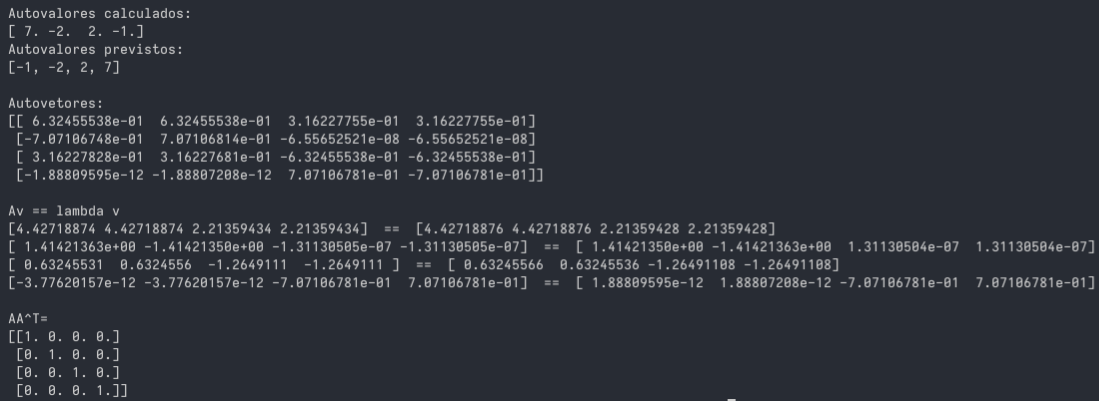
\includegraphics[width=\linewidth]{2021-07-18-12-59-25.png}
\end{center}
o que nos indica que, de fato, o algoritmo está correto.

\section{Tarefa B}

O output dessa tarefa é muito extenso, portanto vamos omití-lo aqui, porém é
facilmente perceptível que este também está correto, i.e.:
\begin{center}
	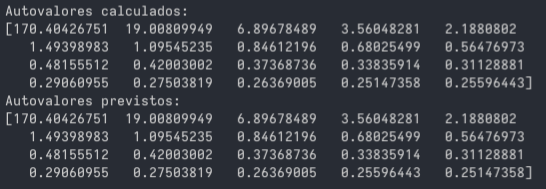
\includegraphics[width=\linewidth]{2021-07-18-12-59-46.png}
	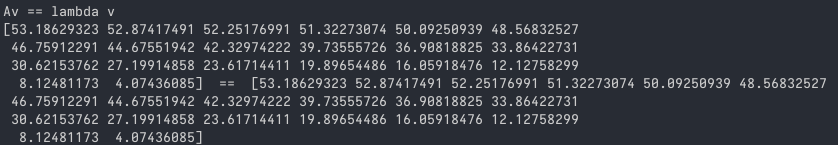
\includegraphics[width=\linewidth]{2021-07-18-12-46-33.png}
	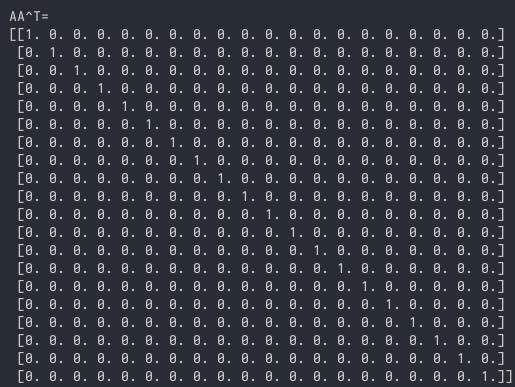
\includegraphics[width=\linewidth]{2021-07-18-12-46-49.png}
\end{center}


\section{Treliça plana}

A tarefa da treliça plana baseia-se na ideia de que as equações de movimento de
cada vértice do objeto podem ser resolvidas por meio de um problema de
autovalores, os quais buscamos otimizar nesse exercício-programa.

Dessa forma nota-se que, após gerar o K estrutural pelo algoritmo iterativo,
podemos aplicá-lo ao mesmo algoritmos das outras duas tarefas para termos a
solução pedida.

Novamente, podemos primeiro observar que nossos testes confirmam o resultado:
\begin{center}
	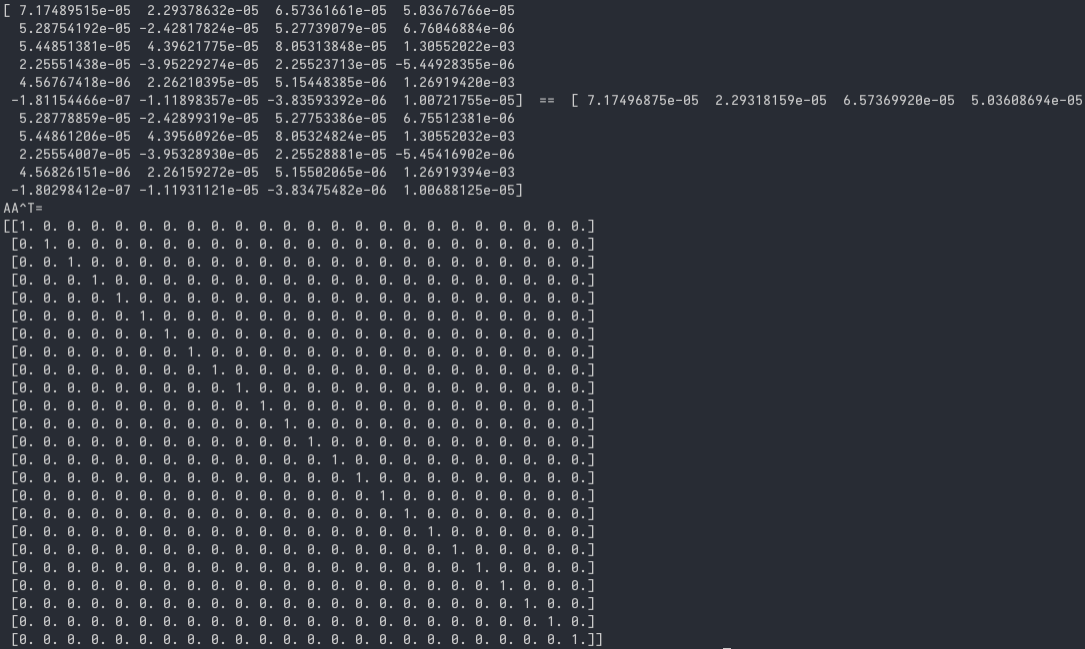
\includegraphics[width=\linewidth]{2021-07-21-19-10-26.png}
\end{center}

E então prosseguimos mostrando o que é pedido:

\begin{center}
	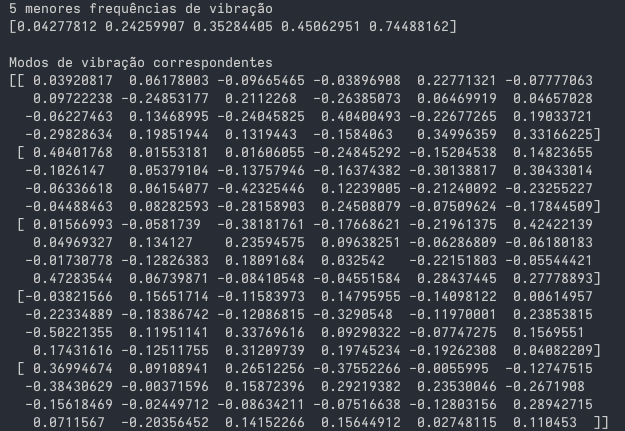
\includegraphics[width=\linewidth]{2021-07-21-19-13-00.png}
\end{center}

\postextual

%\nocite{*}
%\bibliography{bioP1}

% ----------------------------------------------------------
% Glossário
% ----------------------------------------------------------
%
% Consulte o manual da classe abntex2 para orientações sobre o glossário.
%
%\glossary

% ----------------------------------------------------------
% Apêndices
% ----------------------------------------------------------

% ---
% Inicia os apêndices
% ---
%\begin{apendicesenv}
%
%% Imprime uma página indicando o início dos apêndices
%\partapendices
%
%% ----------------------------------------------------------
%\chapter{Quisque libero justo}
%% ----------------------------------------------------------
%
%\lipsum[50]
%
%% ----------------------------------------------------------
%\chapter{Nullam elementum urna vel imperdiet sodales elit ipsum pharetra ligula
%ac pretium ante justo a nulla curabitur tristique arcu eu metus}
%% ----------------------------------------------------------
%\lipsum[55-57]
%
%\end{apendicesenv}
% ---


% ----------------------------------------------------------
% Anexos
% ----------------------------------------------------------

% ---
% Inicia os anexos
% ---
%\begin{anexosenv}
%
%% Imprime uma página indicando o início dos anexos
%\partanexos
%
%% ---
%\chapter{Morbi ultrices rutrum lorem.}
%% ---
%\lipsum[30]
%
%% ---
%\chapter{Cras non urna sed feugiat cum sociis natoque penatibus et magnis dis
%parturient montes nascetur ridiculus mus}
%% ---
%
%\lipsum[31]
%
%% ---
%\chapter{Fusce facilisis lacinia dui}
%% ---
%
%\lipsum[32]
%
%\end{anexosenv}

%---------------------------------------------------------------------
% INDICE REMISSIVO
%---------------------------------------------------------------------
%\phantompart
%\printindex
%---------------------------------------------------------------------

\end{document}
